\chapter{Functions}
\section{What is a function?}
A function takes an input, does something to it, then gives an output. For example:
\begin{example}
If the function "add two" is given 4 as an input it would give 6 as its output.

We will represent this function as \(f(x)=x+2\).
\end{example}

\begin{example}
The human population of the world $P$ depends on the time $t$. The table below gives estimates of the world population at time $t$, for certain years:
\begin{center}
    \begin{tabular}{ | c | c | c | c | c | c | c |}
    \hline
    $t$ (years) & 1900 & 1910 & 1950 & 1960 & 1990 & 2000  \\ \hline
    $P$ (millions) & 1650 & 1750 & 2650 & 3040 & 5280 & 6080  \\ \hline
    \end{tabular}
\end{center}
For instance, $P(1950)\approx 2,560,000,000$ and $P(2000)\approx 6,080,000,000$.

For each value of time $t$, there is a corresponding value of $P$, and we say that $P$ is a function of $t$.

However, in this case we don't know the rule that connects $t$ and $P$ at the moment. In fact, it is one of our tasks to find and understand the rule for a function.
\end{example}

\section{The definition of a function}
Here we will look at more precise definition of a function. First let us define a set.

\begin{definition}
A {\bf set} is a collection of objects, often numbers. An object in a set is called an element of the set.

Sets are written as a list of items inside curly braces (\{ and \}).

If an object \(x\) is in a set \(A\), we will write \(x\in A\).
\end{definition}

\begin{example}
The following are examples of sets:
\begin{itemize}
\item[(i)] $A=\{1,2,8\}$ is a set containing the numbers 1, 2 and 8. We could write \(8\in A\) and \(4\not\in A\);
\item[(ii)] $\mathbb{Z}=\{\text{all whole numbers}\}=\{\dots,-2,-1,0,1,2,\dots\}$;
\item[(iii)] $\mathbb{N}=\{\text{all positive whole numbers}\}=\{0,1,2,3,\dots\}$;
\item[(iv)] $\mathbb{R}=\{\text{all real numbers}\}.$
\end{itemize}
\end{example}

\begin{definition}
If we have two sets $A$ and $B$, then a \textbf{function} $f:A\rightarrow B$ is a rule that sends each element $x$ in $A$ to exactly one element called $f(x)$ in $B$.

We call the set $A$ the \textbf{domain} of $f$. The \textbf{range} of $f$ is the set of all values which $f$ gives as an output ($B$ or a subset of $B$).

If $x\in A$ then $x$ is called an \textbf{independent variable}.
If $y$ is in the range of $f$ then $y$ is called a \textbf{dependent variable}.

\note{$f$ is not a function if it is multi-valued, i.e. if one element from $A$ maps to two distinct elements in $B$. Such a mapping is sometimes called multi-valued function, however this is just terminology, strictly by the definition for our purposes $f$ would not be a function in this case.}
\end{definition}

\section{Representing a function}
Functions are sometimes represented by mapping diagrams:
\begin{figure}[H]
\centering
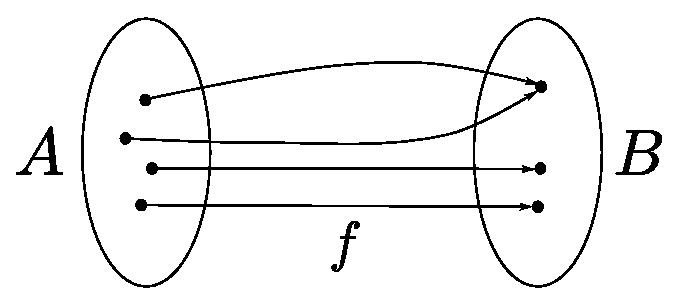
\includegraphics[scale=0.75]{img/function-set}
\captionstyle{\centering\it}
\caption{Function $f$ `maps' elements from set $A$ on to elements in set $B$. Many-to-one relationship. }
\label{fig:function-set}
\end{figure}

The mapping diagram shows the domain and range of the function. The arrows show where is member of \(A\) is sent by the function.

\begin{definition}
Let \(f:A\rightarrow B\) be a function.

If, whenever \(x\) and \(y\) are in \(A\) and not equal, \(f(x)\) and \(f(y)\) are not equal, the function is called \textbf{one-to-one}.

If there are an \(x\) and a \(y\) in \(A\) which are not equal, but \(f(x)\) and \(f(y)\) are equal, the function is called \textbf{many-to-one}.
\end{definition}

\begin{definition}
Let \(f:A\rightarrow B\) be a function.

If $f(-x)=f(x)$, $f$ is called an \textbf{even} function.

If $f(-x)=-f(x)$, $f$ is called an \textbf{odd} function.
\end{definition}

\begin{definition}
If $f(x+T)=f(x)$ for all $x$, then we say that $f(x)$ is a \textbf{periodic function} with period $T$.
\end{definition}

\begin{definition}
A function, $f$, has a \textbf{vertical asymptote} at \(x=a\) if as \(x\rightarrow a\), \(f(x)\rightarrow\pm\infty\).

A function, $f$, has a \textbf{horizontal asymptote} at \(y=b\) if as \(x\rightarrow \infty\), \(f(x)\rightarrow b\) or if as \(x\rightarrow -\infty\), \(f(x)\rightarrow b\).
\end{definition}

\begin{example}
Let $S$ be the function from the real numbers to itself, that is $S:\mathbb{R}\rightarrow \mathbb{R}$ given by
\begin{equation}
S(x)=x^2.
\end{equation}
The domain of $S$ is $\mathbb{R}$. As squaring any real number gives a positiveresult, the range of $S$ is $\mathbb{R}^+$ (the set of positive real numbers).

We can write $S(3)=9$ or $S(1.5)=2.25$.

We can also represent some values of $S$ with table of values:
\begin{center}
    \begin{tabular}{ | c | c | c | c | c | c | c |}
    \hline
    $x$  & 1 & 2 & 3 & $\dots$ & 7 & $\dots$  \\ \hline
    $S(x)$ & 1 & 4 & 9 & $\dots$ & 49 & $\dots$  \\ \hline
    \end{tabular}
\end{center}

Functions are often represented visually, as graphs.

\begin{figure}[H]
\centering
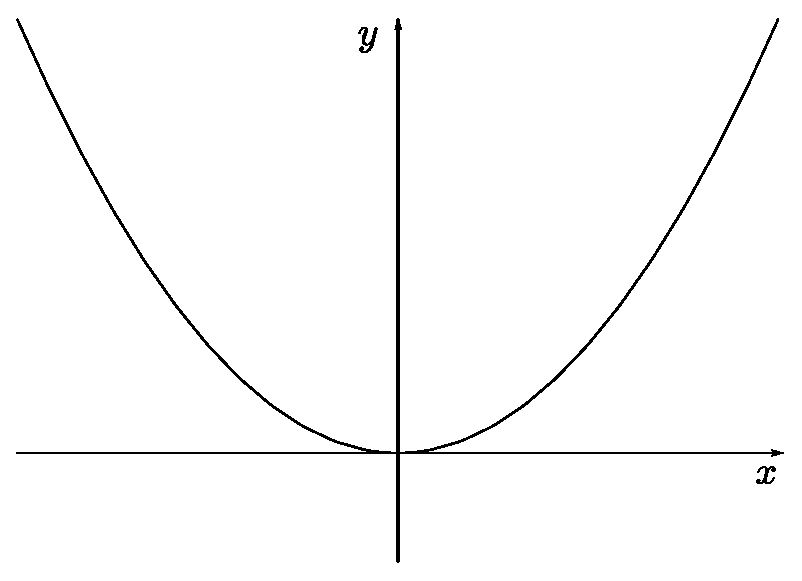
\includegraphics[scale=0.65]{img/x-squared-graph}
\captionstyle{\centering\it}
\caption{Graph displaying the function $y=S(x)=x^2$.}
\label{fig:x-squared-graph}
\end{figure}
\end{example}

\section{Polynomials}
\begin{definition}
A polynomial is a function $P$ with a general form
\begin{equation}
P(x)=a_0 + a_1x + a_2x^2+\dots+a_nx^n,
\end{equation}
where the coefficients $a_i$ $(i=0,1,\dots,n)$ are numbers and $n$ is a non-negative whole number. The highest power whose coefficient is not zero is called the \textbf{degree} of the polynomial $P$.
\end{definition}

\begin{example}
\hspace{1em}
\begin{center}
    \begin{tabular}{ | c | c | c | c | c | c | c |}
    \hline
    $P(x)$  & 2 & $3x^2+4x+2$ & $\frac{1}{1+x}$ & $\sqrt{x}$ & $1-3x+\pi x^3$ & $2t+4$  \\ \hline
    \textbf{Polynomial?} & Yes & Yes & No & No & Yes & Yes  \\ \hline
    \textbf{Order} & 0 & 2 & N/A & N/A & 3 & 1  \\ \hline
    \end{tabular}
\end{center}
\end{example}

\subsection{Some polynomial degrees}
\subsubsection{Degree 0} $P_0(x)=a_0x^0=a_0,$ say $P(x)=2$. This polynomial is simply a constant.
\begin{figure}[H]
    \hspace{0.2cm}
    \subfigure[$y=P(x)=2$.]{\label{fig:y-2-const-graph}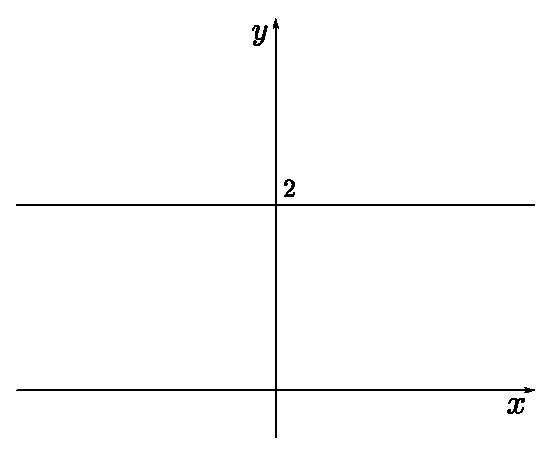
\includegraphics[scale=0.6]{img/y-2-const-graph}}
    \hspace{2.0cm}
    \subfigure[{\it Entire domain mapped to one point.}]{\label{fig:y-2-const-set}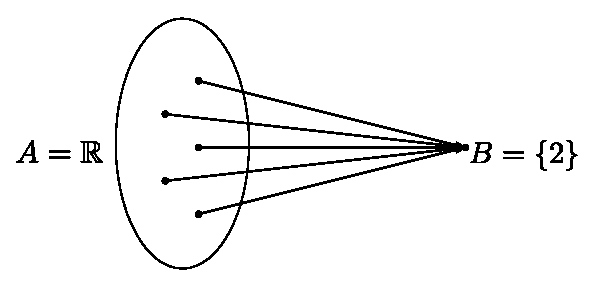
\includegraphics[scale=0.6]{img/y-2-const-set}} \\
    \centering
  \caption{{\it A degree 0 polynomial.}}
  \label{fig:exponent-graphs}
\end{figure}

\subsubsection{Degree 1} $P_1(x)=a_0x^0+a_1x^1 = ax+b$ ($a\ne 0$). These are called {\it linear}, since the graph of $y=ax+b$ is a straight line. The linear equation $ax+b=0$ has solution $x=-b/a$.\\
\begin{figure}[H]
\centering
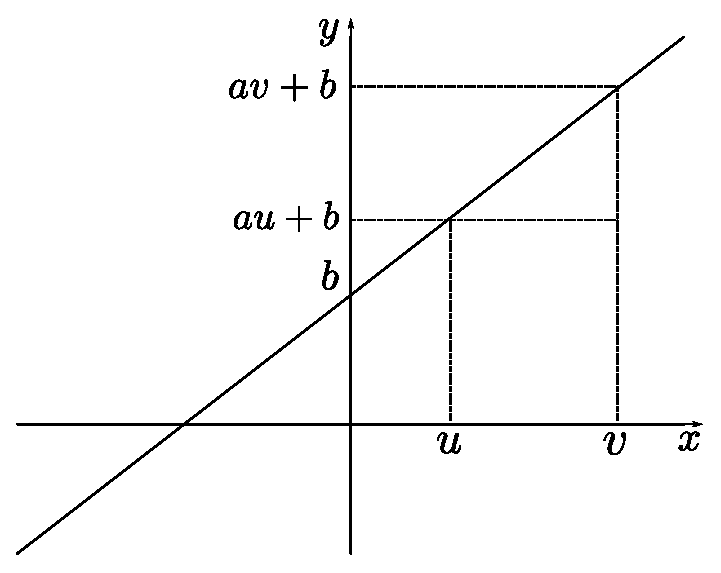
\includegraphics[scale=0.65]{img/linear-graph}
\captionstyle{\centering\it}
\caption{Linear graph given by $y=ax+b$.}
\label{fig:linear-graph}
\end{figure}

The \textbf{gradient} of $y=ax+b$ is $a$. It can be worked out as follows:
\begin{eqnarray}
\text{gradient} &=& \frac{\text{change in height}}{\text{change in distance}} \nonumber \\
&=& \frac{\text{change in }y}{\text{change in }x} \nonumber \\
&=& \frac{(av+b)-(au+b)}{v-u} \nonumber \\
&=& \frac{a(v-u)}{v-u} = a.
\end{eqnarray}

